% !TeX spellcheck = ru_RU
% !TEX root = vkr.tex

\section{Эксперимент}

В данном разделе представлены результаты экспериментального исследования алгоритма, описанного в предыдущих главах. Основные задачи исследования --- оценить производительность BFS с использованием линейной алгебры и многопоточности в условиях, близких к реальным, сравнить полученные показатели и ответить на вопросы, приведённые ниже.

\begin{itemize}
    \item[\textbf{RQ1:}] При каких параметрах графа выгоднее использовать параллельную версию алгоритма, а при каких последовательную?
    \item[\textbf{RQ2:}] Использование какого количества потоков даёт наибольший выигрыш в производительности?
    \item[\textbf{RQ3:}] Чем можно объяснить полученное количество потоков, дающих наибольший выигрыш в производительности?
\end{itemize}

\subsection{Условия эксперимента}

Эксперименты проводились на рабочей станции со следующими характеристиками.
\begin{itemize}
    \item Центральный процессор: AMD Ryzen 5 5600X 
    \item Количество ядер ЦПУ: 6 ядер, 12 потоков 
    \item Операционная система: Windows 11 Pro, version 22H2
\end{itemize}

\subsection{Набор данных}

Для замеров производительности использовались неориентированные графы, т.~е. графы с симметричной матрицей смежности. Примеры реальных данных взяты из коллекции университета Флорида \cite{10.1145/2049662.2049663}. Из них были выбраны 5 разреженных матриц различного порядка, количество ненулевых элементов которых не превышает 1.34\%. В табл. \ref{tbl:matrices} представлена информация об используемых данных: название, порядок, количество ненулевых элементов и плотность --- отношение числа ненулевых элементов к общему числу, умноженное на 100.

\begin{table}
\begin{center}
\caption{Разреженные матричные данные}
\label{tbl:matrices}
\rowcolors{2}{black!2}{black!10}
\scalebox{0.7}{
\begin{tabular}{|l|r|r|r|}
\hline
Название &  Порядок & Ненулевые эл-ы & Плотность \\
\hline
\hline
HB/bcsstm03                     & 112            & 72           & 0.57 \\
HB/dwt\_512                     & 512            & 3,502        & 1.34 \\
Gset/G52                        & 1,000          & 11,832       & 1.18 \\
Gset/G59                        & 5,000          & 59,140       & 0.24 \\
ML\_Graph/kmnist\_norm\_10NN    & 10,000         & 156,932      & 0.15 \\
\hline
\end{tabular}
}
\end{center}
\end{table}

В данной работе результат работы BFS не зависит от типа меток на рёбрах (в ответе учитывается только порядок посещения вершин), поэтому все матрицы, взятые в качестве экспериментальных данных, будут обрабатываться как матрицы Pattern-типа. Такой выбор обусловлен тем, что арифметические операции с одними примитивными типами могут быть более ресурсоёмкий по сравнению с другими (в данном случае в сравнении с типами Real и Integer).

\subsection{Метрики}

В экспериментальном исследовании для замеров производительности была использована библиотека Bench\-mark\-Dot\-Net~v0.13.4\footnote{Библиотека BenchmarkDotNet для замеров производительности: \url{https://benchmarkdotnet.org/}.}. В качестве метрик производительности выступает время, требуемое для выполнения операции. Стандартное отклонение (StdDev) составляет не более 10\% от среднего значения (mean) для каждого отдельного эксперимента.

\subsection{Результаты}

Столбчатые диаграммы на рис. \ref{fig:barPlot112},\ref{fig:barPlot1000},\ref{fig:barPlot5000},\ref{fig:barPlot10000},\ref{fig:barPlot50000} реализованные с помощью инструмента Matplotlib \cite{Hunter:2007}, иллюстрируют результаты экспериментального исследования. На оси абсцисс отмечены уровни параллельности, представленные в формате (\texttt{multiLe\-vel}, \texttt{addMultiLevel}, \texttt{addLevel}), на оси ординат --- отношение среднего значения на базовом уровне (0,0,0) к среднему значению на текущем уровне параллельности, далее именуемое \textit{ускорением}. Столбцы окрашены в соответствии с цветовой картой  \enquote{viridis} таким образом, что оттенки цветов (от фиолетового до жёлтого) соотносятся с ускорением --- чем больше, тем правее по спектру. Красным выделены уровни, при которых время работы алгоритма оказалось наименьшим. Горизонтальная пунктирная линия проведена на уровне базового значения и помогает визуально сравнить с ним другие показатели.

\textit{RQ1: При каких параметрах графа выгоднее использовать параллельную версию алгоритма, а при каких последовательную?}

В трёх из пяти случаях, оказалось выгоднее использовать параллельную версию алгоритма, а именно в графах с матрицами смежности порядка 1000, 5000 и 10000. В графах с меньшими (относительно остальных) размерами 112 и 512 параллельные версии обхода в ширину не ускоряли, а, наоборот, замедляли процесс. Наилучший показатель (на уровне (0,0,1)) параллельной версии алгоритма на матрице порядка 112 примерно в 2.9 раз медленнее базового значения; на матрице порядка 512 --- в 1.6 раз (на уровне (0,0,1)). Такой результат можно объяснить тем, что на накладные расходы, приведённые в обзоре, и параллельное выполнение суммарно тратиться больше времени, чем на работу однопоточной версии.

\textit{RQ2: Использование какого количества потоков даёт наибольший выигрыш в производительности?}

Ответ на исследовательский вопрос RQ2 представлен в табл. \ref{tbl:bestscore}.

\begin{table}
\begin{center}
\caption{Уровни, дающие наибольший выигрыш}
\label{tbl:bestscore}
\rowcolors{2}{black!2}{black!10}
\scalebox{0.7}{
\begin{tabular}{|l|r|r|r|r|r|}
\hline
Название &  Порядок & multiLevel & addMultiLevel & addLevel & Ускорение\\
\hline
\hline
Gset/G52                        & 1,000          & 2            & 0       & 2  & 3.45\\
Gset/G59                        & 5,000          & 3            & 0       & 0  & 2.65\\
ML\_Graph/kmnist\_norm\_10NN    & 10,000         & 2            & 0       & 4  & 3.21\\
\hline
\end{tabular}
}
\end{center}
\end{table}

\begin{figure}
    \centering
    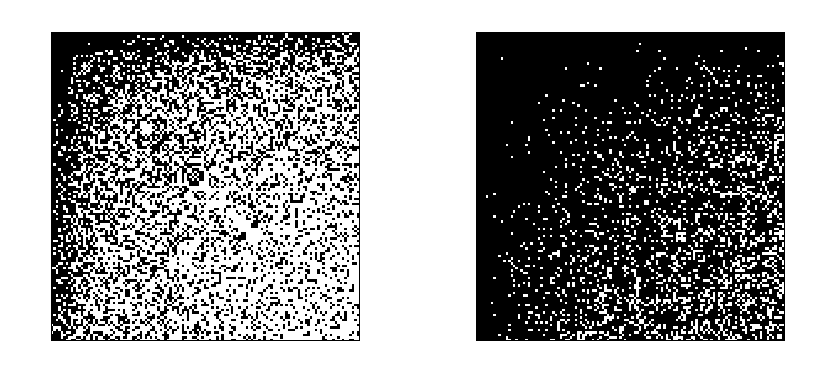
\includegraphics[width=\textwidth]{matrices.png}
    \caption{Визуализация разреженности матрицы порядка 1000 (слева) и порядка 5000 (справа)}
    \label{fig:mtx}
\end{figure}

\textit{RQ3:  Чем можно объяснить полученное количество потоков, дающих наибольший выигрыш в производительности?}

Как было упомянуто ранее, на каждом уровне параллельности умножения создаётся по 4 задачи и по 2 --- на каждом уровне сложения. Таким образом,  имея параметры (2,0,2), мы получим суммарно 21 задачу для умножения и 13 задач для сложения; задачи умножения могут распределиться между 12 потоками не более чем по две на каждый, что может быть обосновано высказанным раннее утверждением об эффективности переключении процессора между задачами, находящимися в одном потоке.

Действительно, вновь обращаясь к рис. \ref{fig:uml} можно заметить, что после распределения задач основным потоком, он простаивает в ожидании ответа от потоков 1--2, которые аналогично ожидают потоки 3--6 --- в это время их можно дополнительно нагрузить. Оптимальным является сценарий, при котором задачи, созданные на одном уровне параллельности (1 задача на уровне 0, 4 на уровне 1, 16 на уровне 2 и т.д.), выполнялись бы на максимально возможном количестве потоков. Таким образом, при параметре \texttt{multiLevel = 1} мы получим 4 задачи, которые можно распределить максимум между 4 потоками, а остальные 8 окажутся незанятыми, хотя потенциально на них могли выполняться вычисления. 

Также отметим следующий факт --- чем больше уровень параллельности, тем на более мелкие составляющие разделяется основная задача. В случае, когда вычисление каждой подзадачи занимает меньше времени, чем накладные расходы (например, в области сильной разреженности), выгоднее остановить разбиение. Верно и обратное. Это утверждение может объяснить, почему в матрице размера 5000 выгоднее использовать 3, а не 2 уровня параллельности умножения ---достаточно сравнить количество областей разреженности матрицы размера 1000 и матрицы размера 5000 на рис. \ref{fig:mtx}.

Кроме того, на диаграммах \ref{fig:barPlot1000}, \ref{fig:barPlot5000}, \ref{fig:barPlot10000} видно, что параллельная версия сложения не так эффективна, как параллельная версия умножения --- достаточно сравнить показатели вида (0,0,x) или (0,x,0) и (x,0,0). Однако, может давать небольшой выигрыш, например в случае с матрицами 1000 и 10000.

\begin{landscape}
\begin{figure}
    \thispagestyle{empty} 
    \centering
    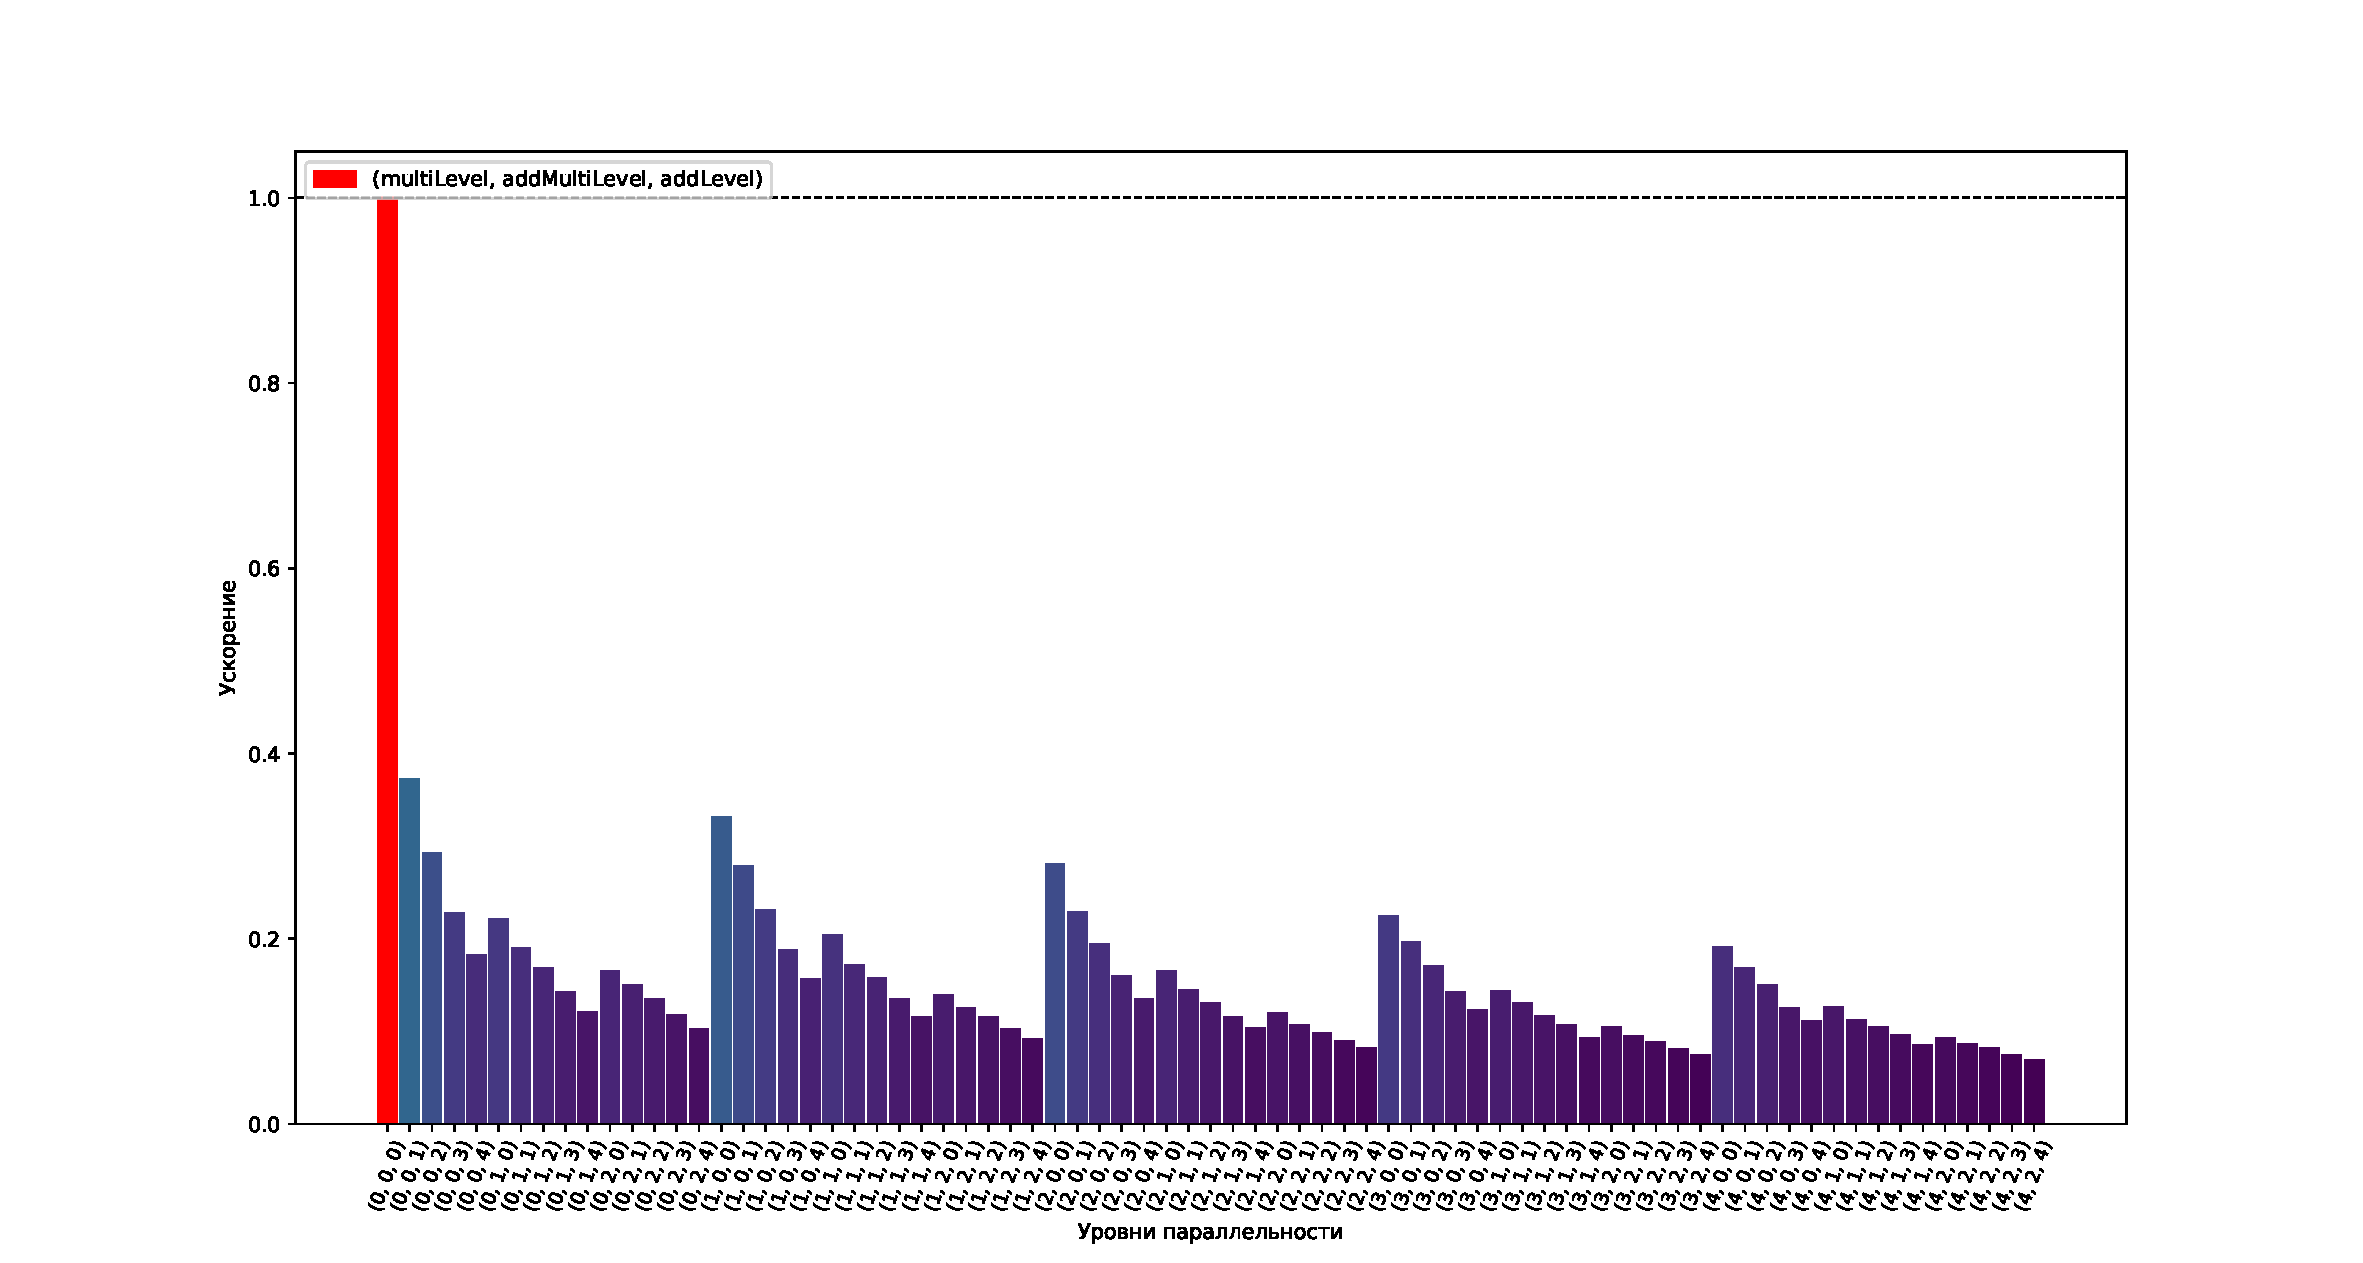
\includegraphics[height=0.8\textwidth]{figures/barPlot112.pdf}
    \caption{Результаты измерения времени работы BFS с различными уровнями параллельности на мат\-ри\-це~HB/bcsstm03 порядка 112\\}
    \label{fig:barPlot112}
\end{figure}
\end{landscape}

\begin{landscape}
\begin{figure}
    \thispagestyle{empty} 
    \centering
    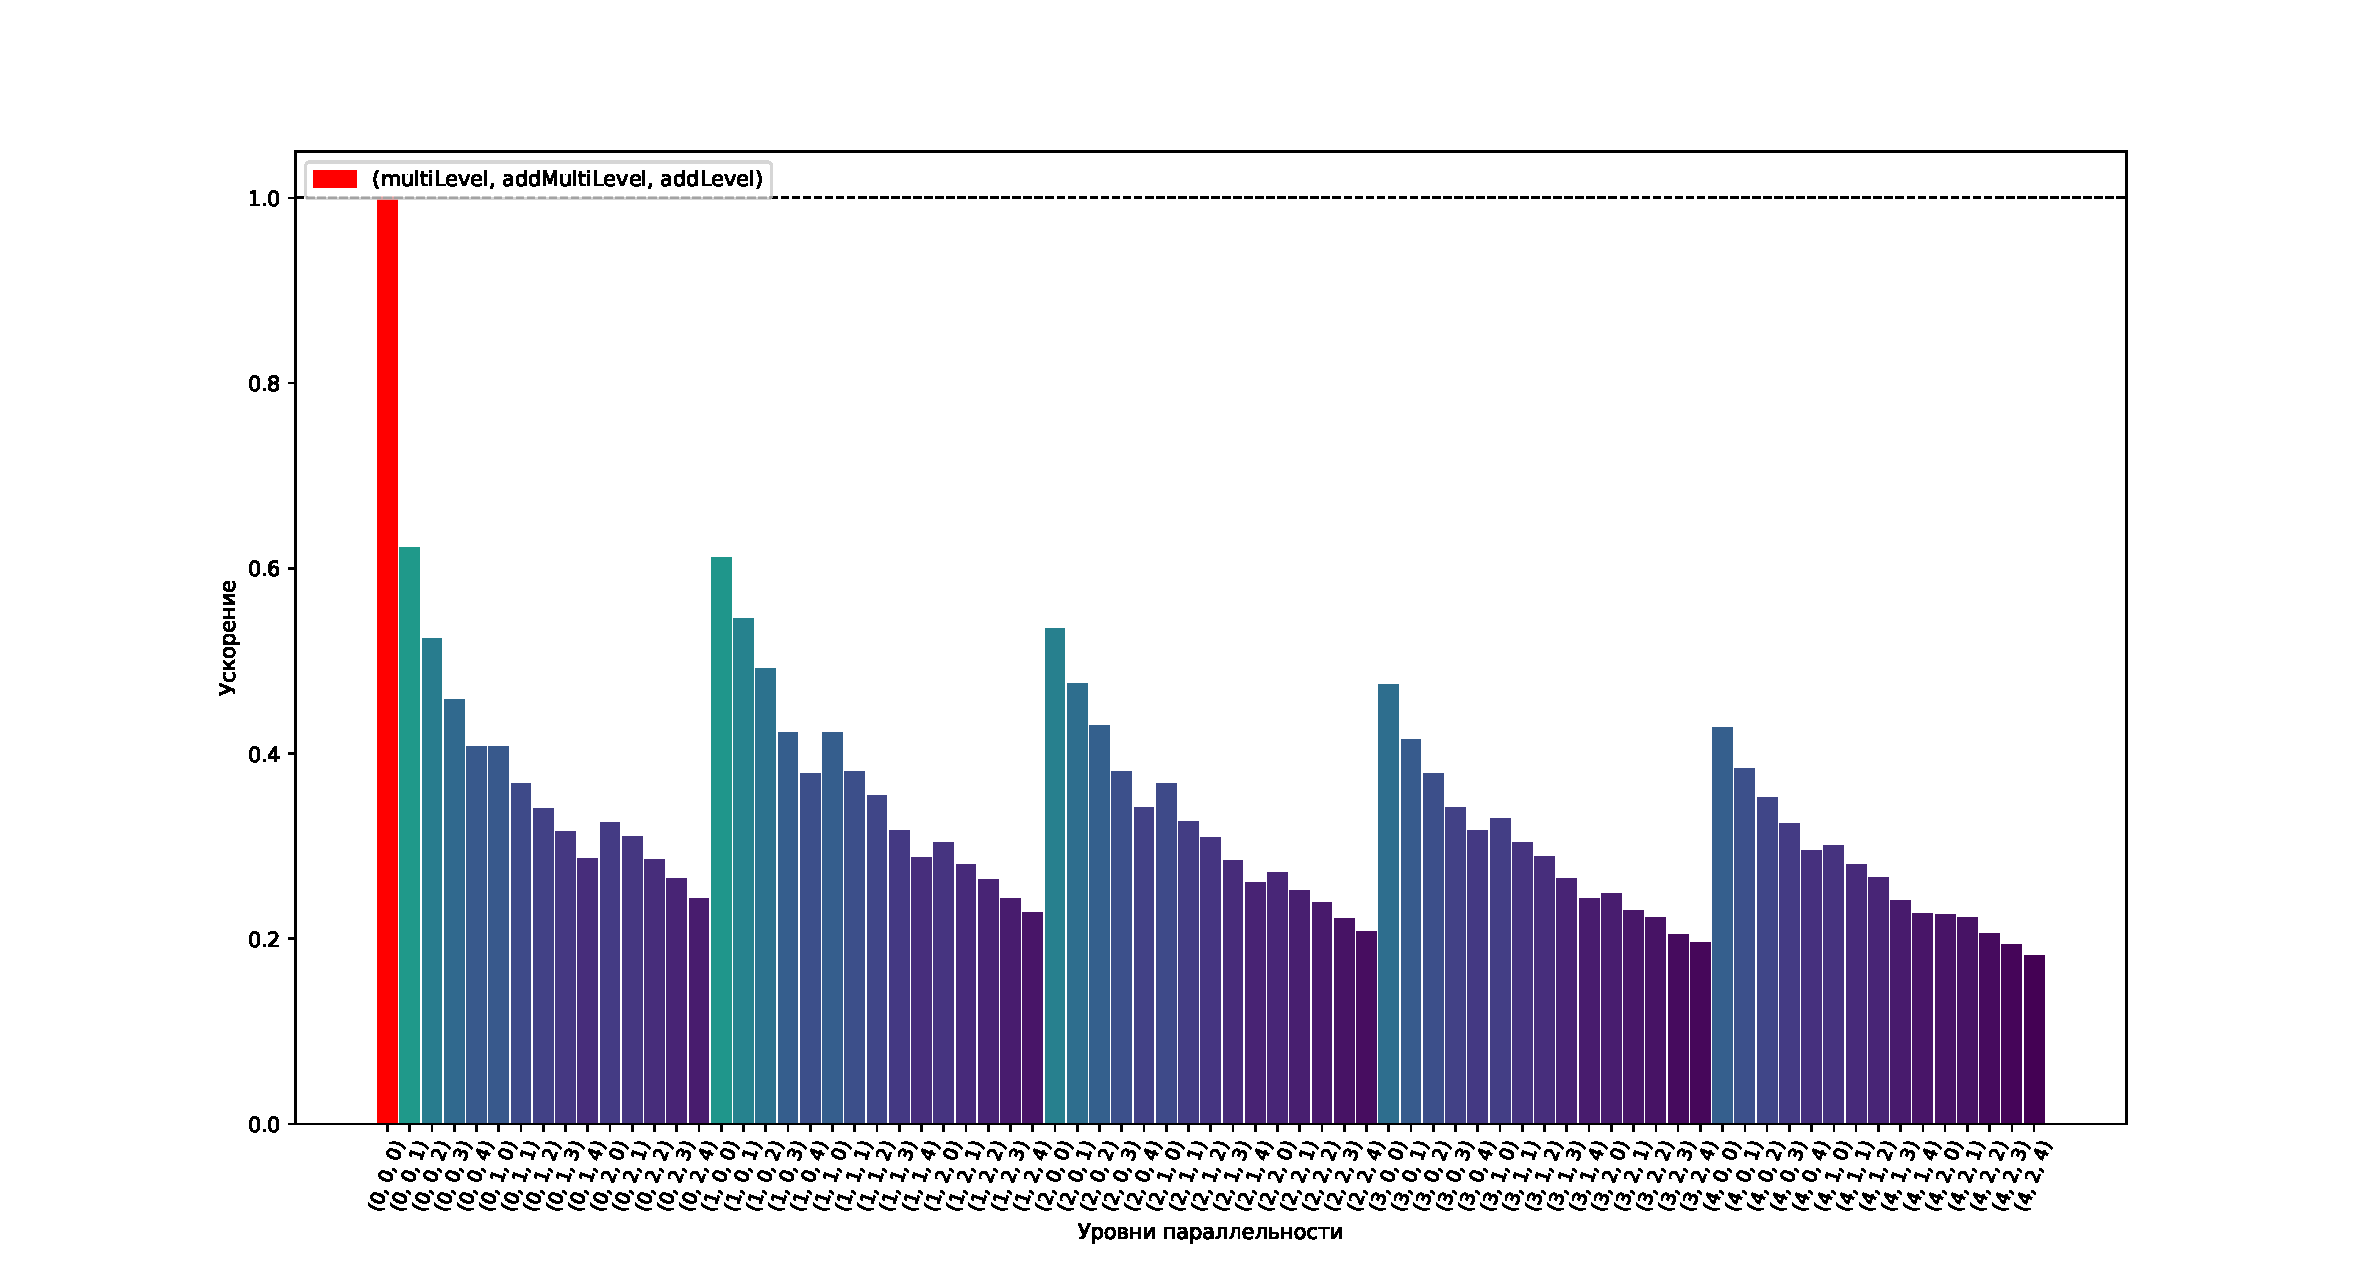
\includegraphics[height=0.8\textwidth]{figures/barPlot512.pdf}
    \caption{Результаты измерения времени работы BFS с различными уровнями параллельности на мат\-ри\-це~HB/dwt\_512 порядка 512\\}
    \label{fig:barPlot50000}
\end{figure}
\end{landscape}

\begin{landscape}
\begin{figure}
    \thispagestyle{empty} 
    \centering
    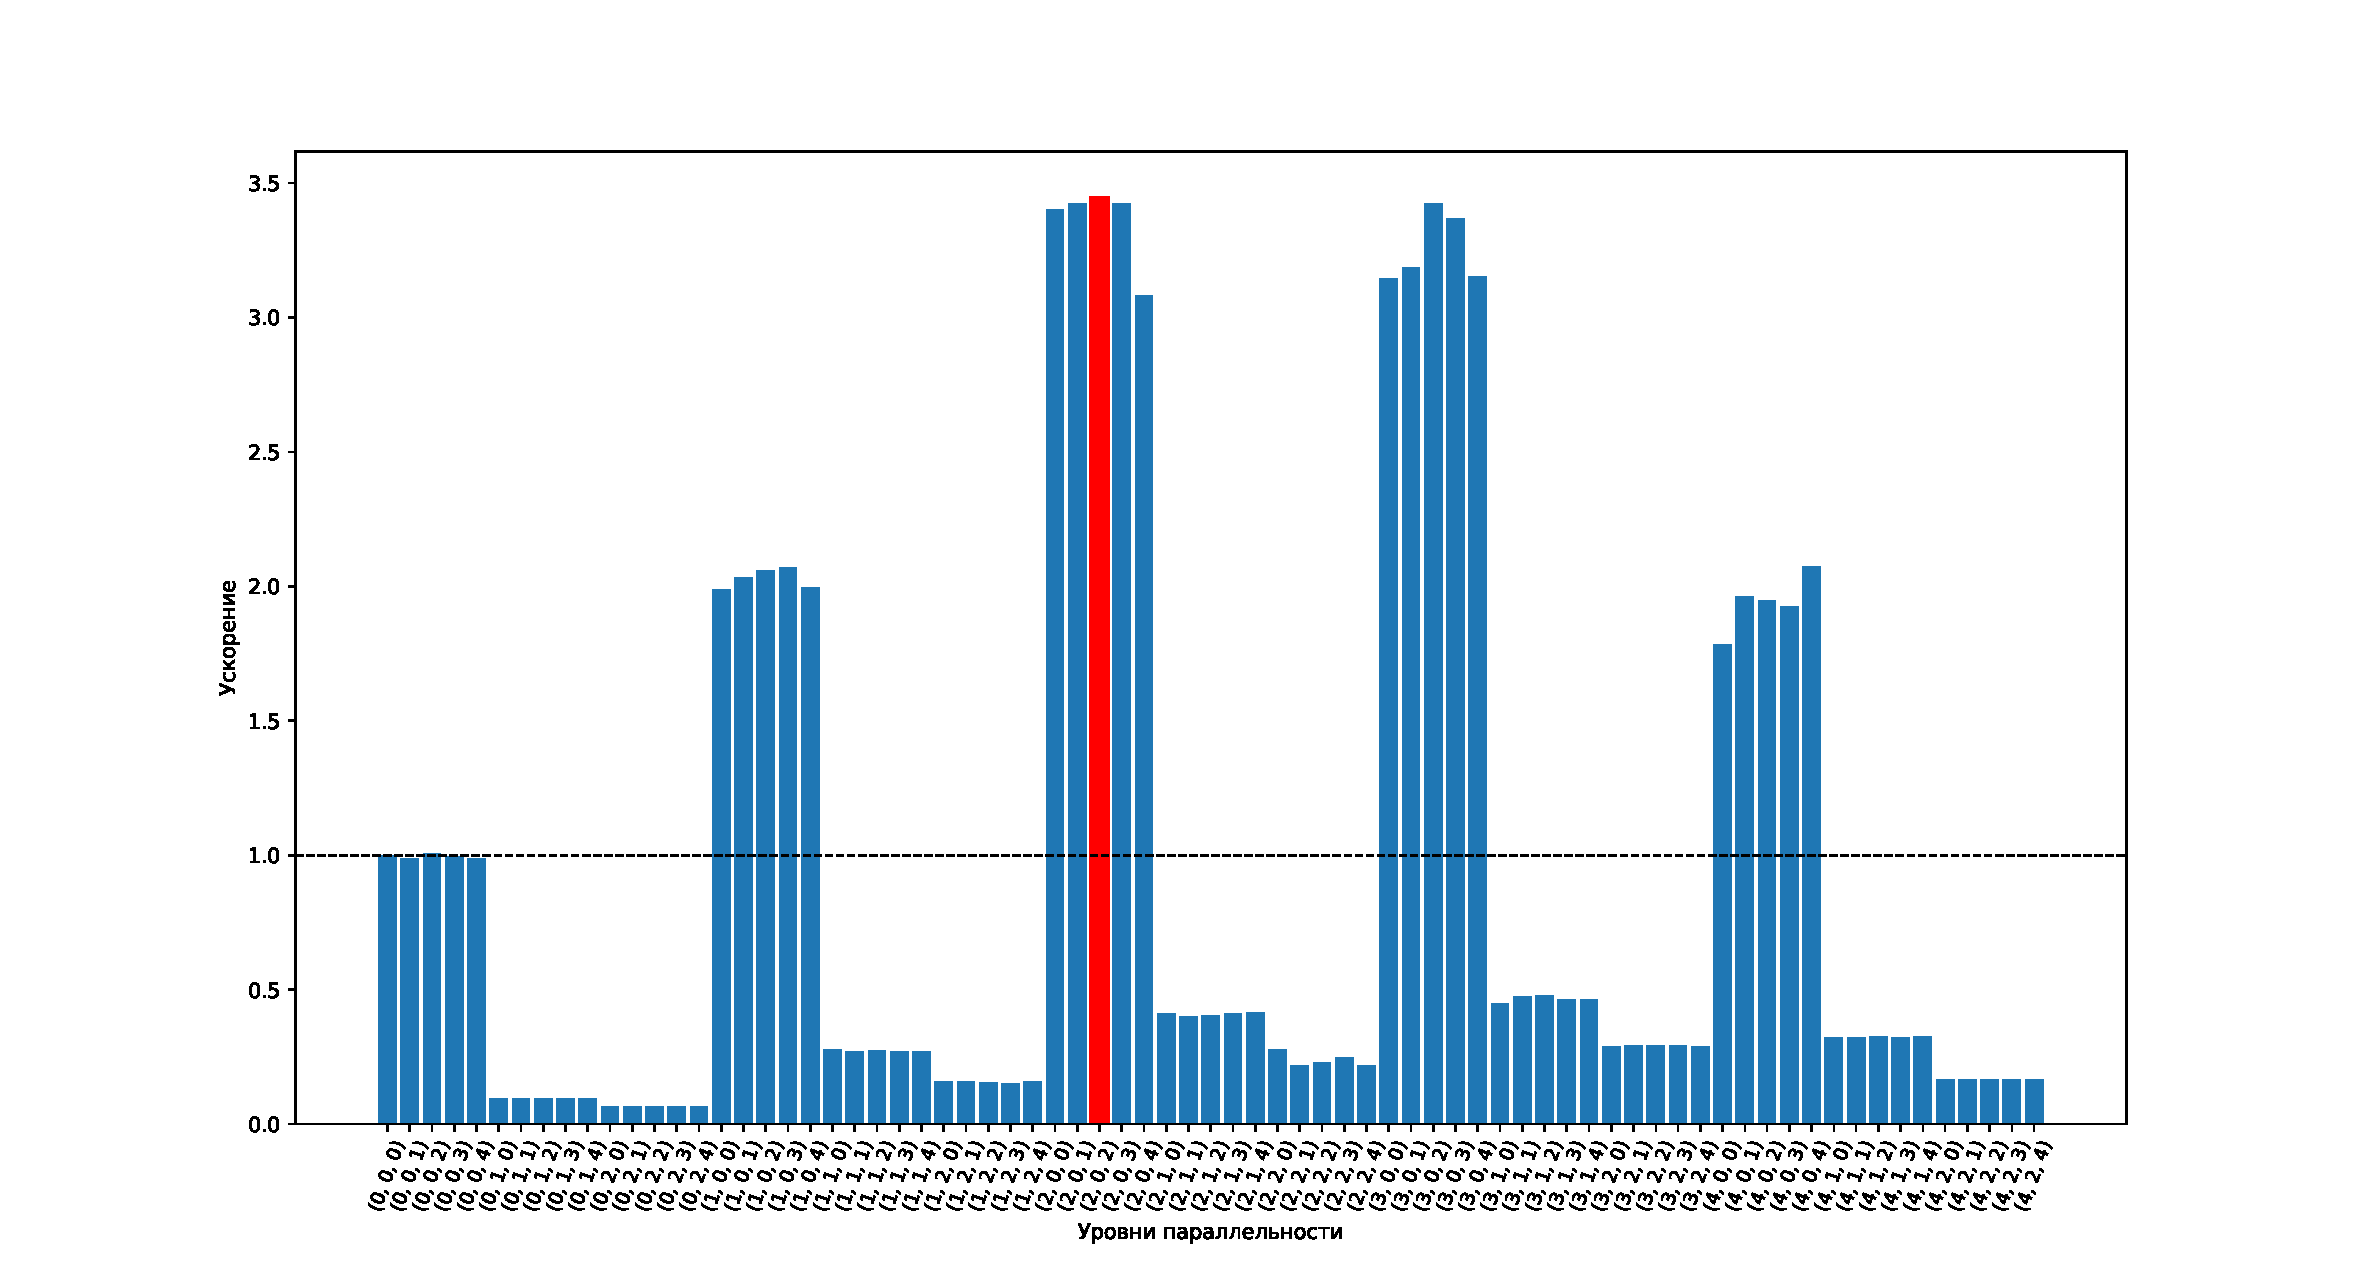
\includegraphics[height=0.8\textwidth]{figures/barPlot1000.pdf}
    \caption{Результаты измерения времени работы BFS с различными уровнями параллельности на мат\-ри\-це~Gset/G52 порядка 1000\\}
    \label{fig:barPlot1000}
\end{figure}
\end{landscape}

\begin{landscape}
\begin{figure}
    \thispagestyle{empty} 
    \centering
    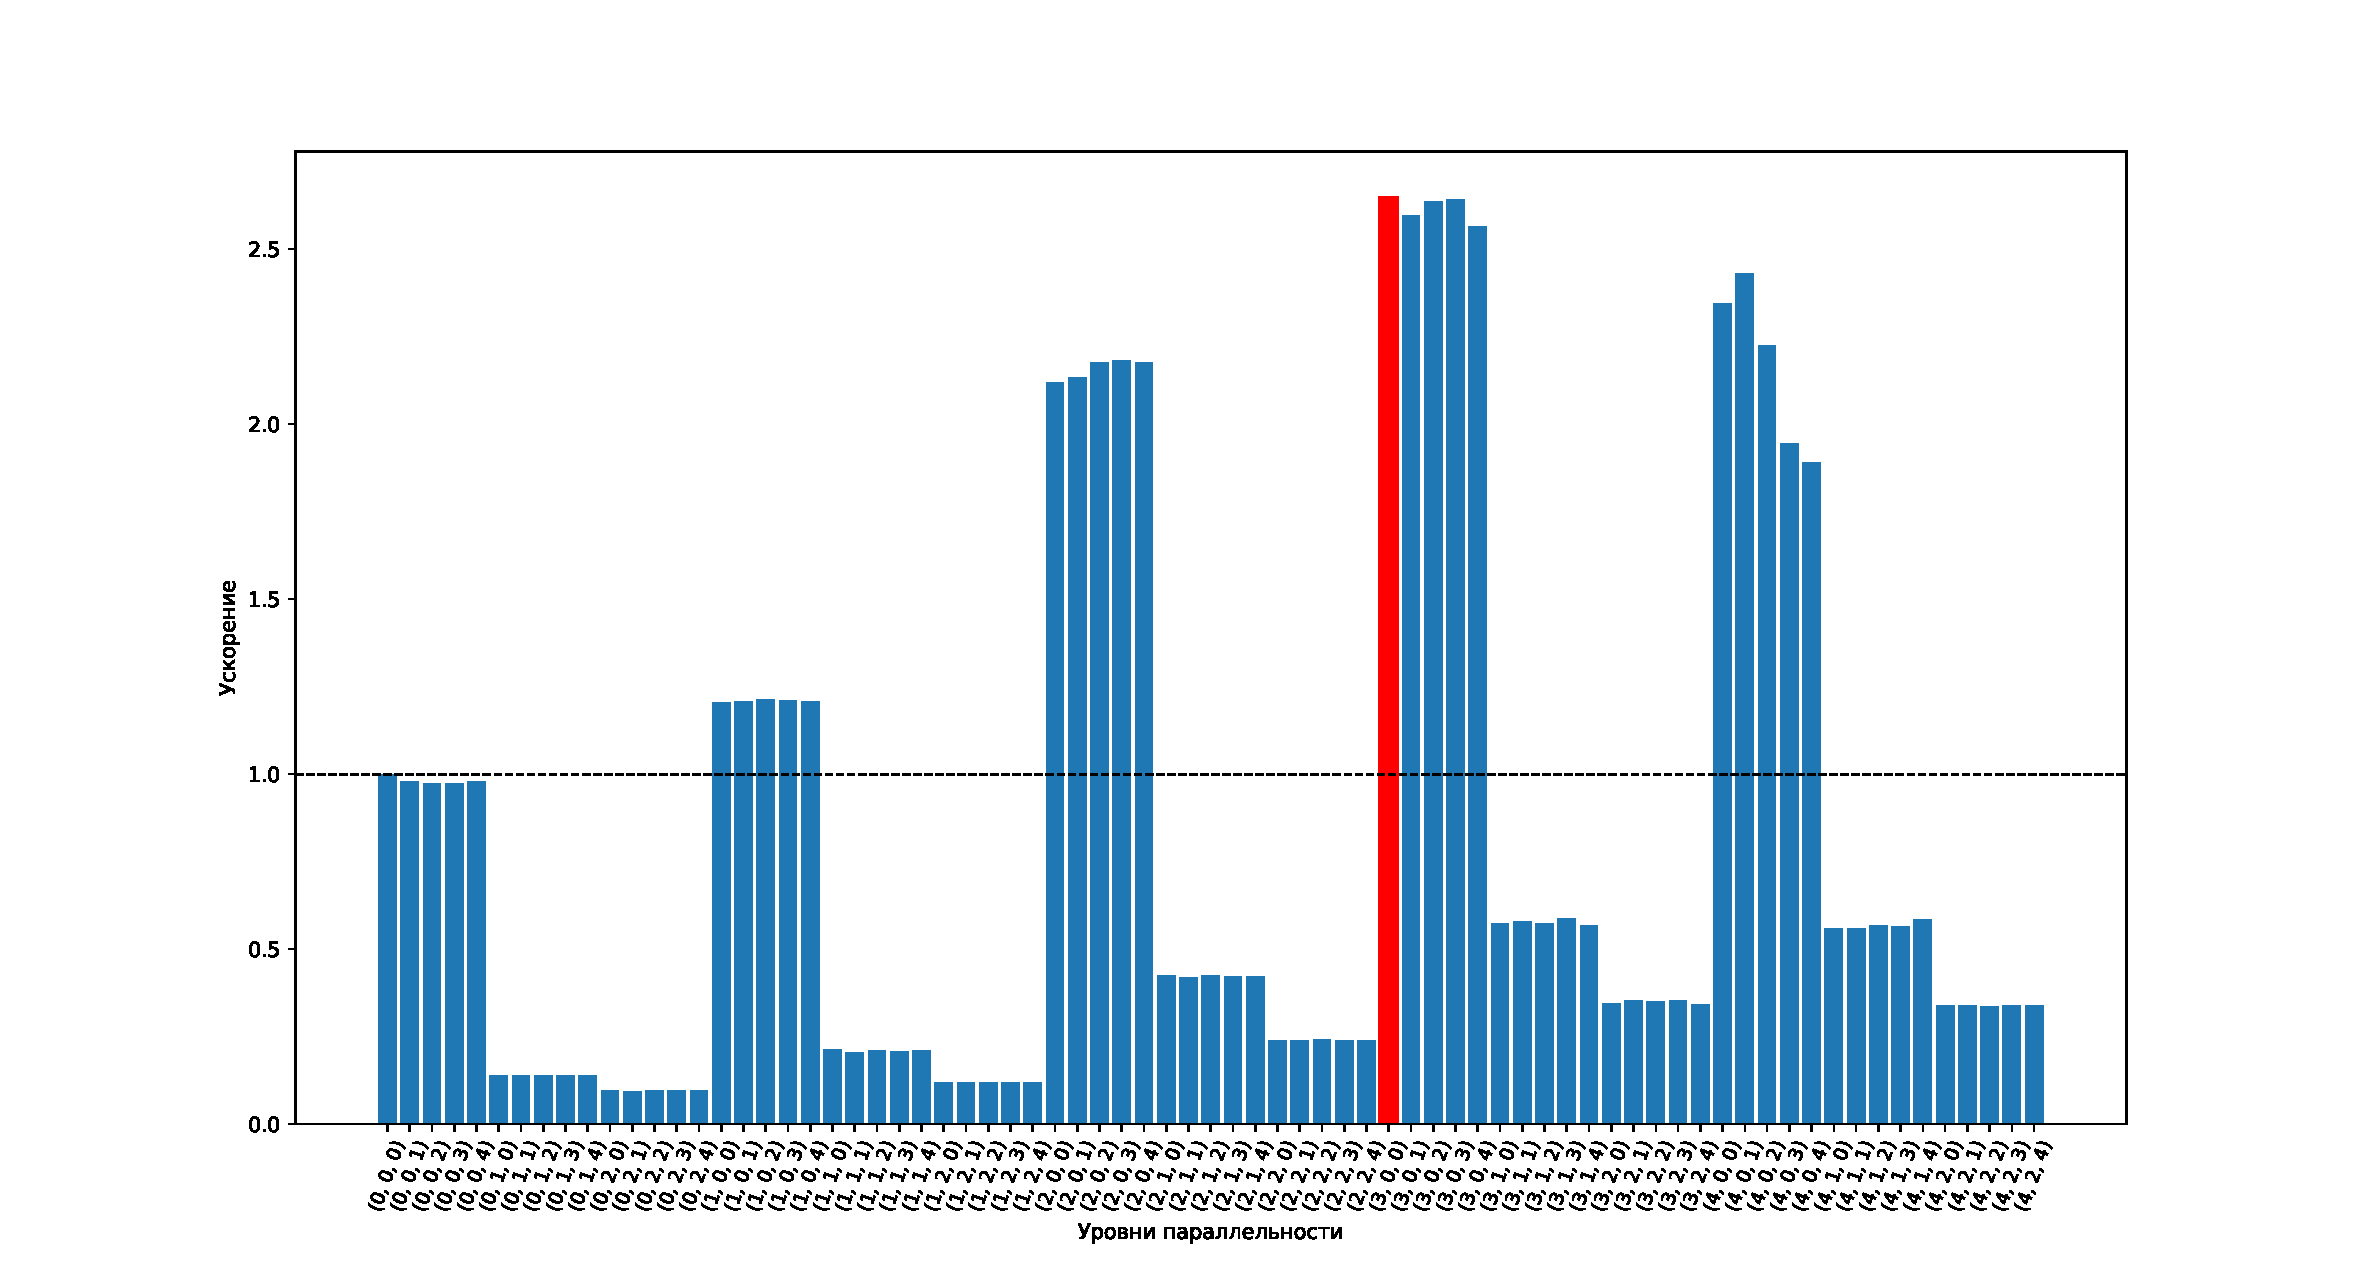
\includegraphics[height=0.8\textwidth]{figures/barPlot5000.pdf}
    \caption{Результаты измерения времени работы BFS с различными уровнями параллельности на мат\-ри\-це~Gset/G59 порядка 5000\\}
    \label{fig:barPlot5000}
\end{figure}
\end{landscape}

\begin{landscape}
\begin{figure}
    \thispagestyle{empty} 
    \centering
    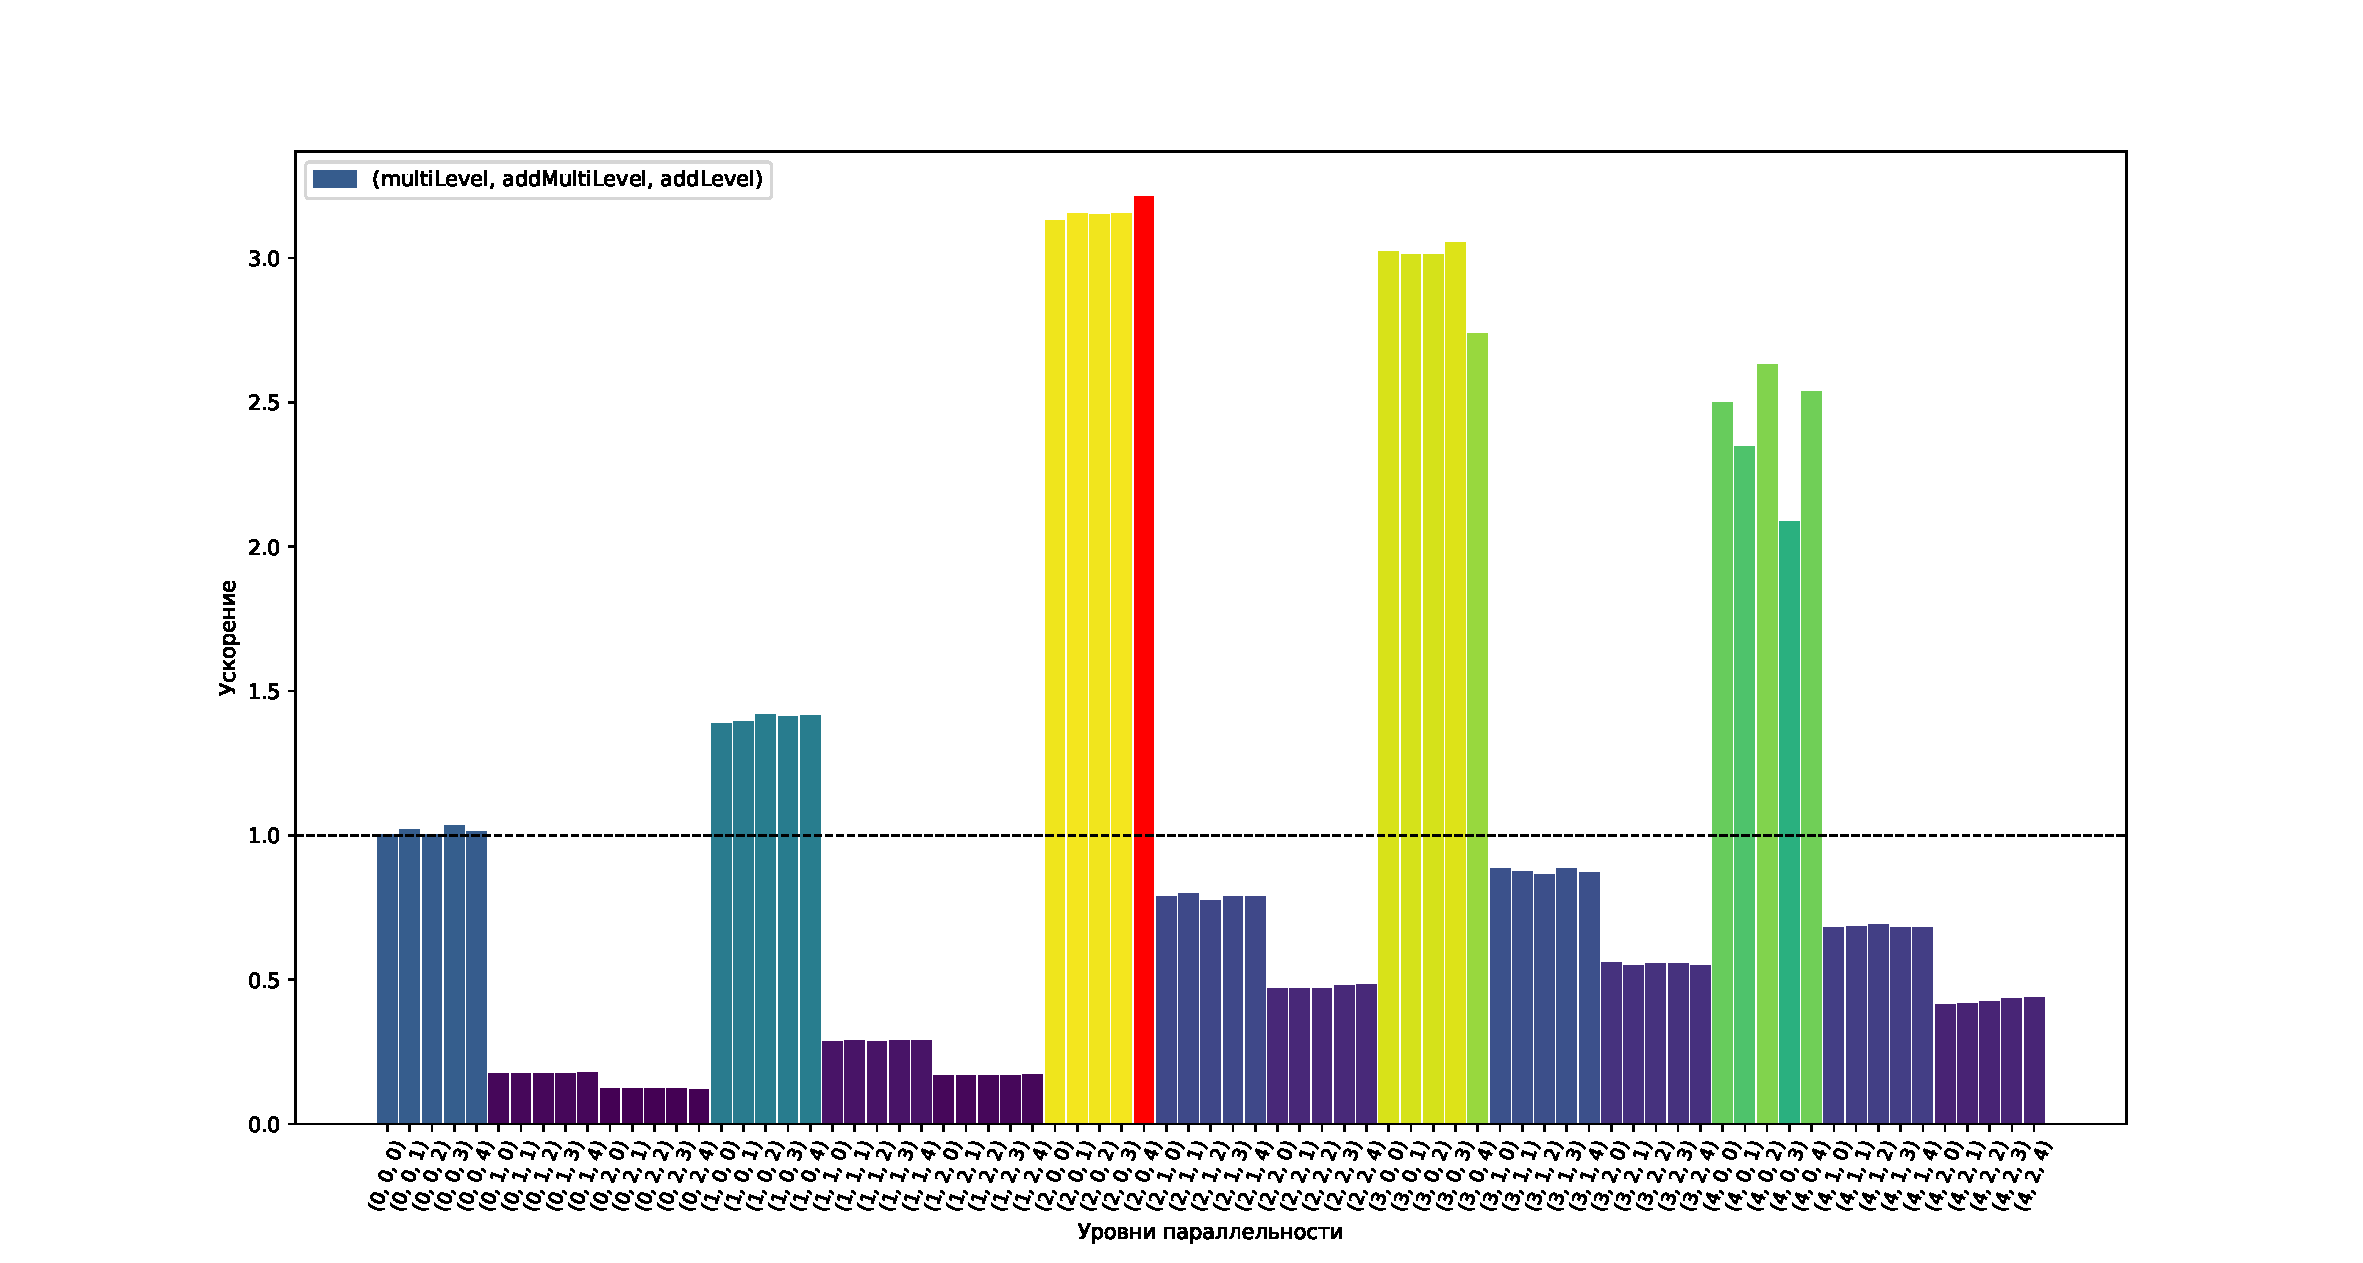
\includegraphics[height=0.8\textwidth]{figures/barPlot10000.pdf}
    \caption{Результаты измерения времени работы BFS с различными уровнями параллельности на мат\-ри\-це~ML\_Graph/kmnist\_norm\_10NN порядка 10000\\}
    \label{fig:barPlot10000}
\end{figure}
\end{landscape}

